\chapter{Data, Features, and Models}
\begin{chapquote}{Kevin P. Murphy}
    ``The goal of machine learning is to develop methods that can automatically detect patterns in data, and then to use the uncovered patterns to predict future data or other outcomes of interest.''
\end{chapquote}

At a basic level, machine learning is about predicting the future based on the past. For instance, you might wish to predict how much a user Alice will like a movie that she hasn't seen, based on her ratings of movies that she has seen. This prediction could be based on many factors of the movies; in general, this means making informed guesses about some unobserved property of some object, based on observed properties of that object.

\section{The learning process}

\begin{figure}[h]
\begin{center}
    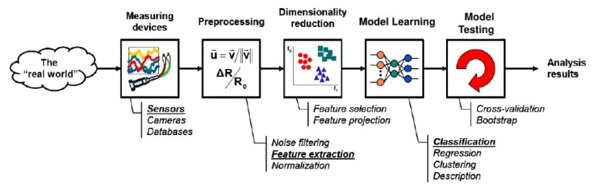
\includegraphics[width=.95\textwidth]{015}
\end{center}
\caption{Learning process scheme}
\label{fig:015}
\end{figure}

From the data we acquire knowledge, which is represented by a model, the model is used on future data.

In Figure~\ref{fig:015} we have a simplified pipeline of the learning process, divided by stages. 

The \textbf{measurement} can come from different sensors or database, these data are obtained in different ways, and then they are preprocessed. 

The \textbf{preprocessing} depends on the application, for example it can be noise filtering for measurements done when working with sensonrs. We need to transform our data in a set of vectore, called \emph{feature}, this operation is called \emph{feature extraction}. It is common, in many application, to do a normalization, which can be achieved in different ways.

Usually, feature extracted from the data are not directly fed into the model, but there is a selection (or projection) of the vectors to \textbf{reduce their dimensionality} and maintaining only useful information. Then, the machine learning algorithm is applied, it can differ depending on the different task of the applcation. Once we have outputted our model from the chosen algorithm, the testing phase is performed.

\section{Data}

\textbf{Data} are individual facts, statistics, or items of information, often numeric. In a more technical sense, data are a set of values of qualitative or quantitative variables about one or more persons or objects, while a \emph{datum} is a single value of a single variable.

\begin{wrapfigure}{r}{0.35\textwidth}
      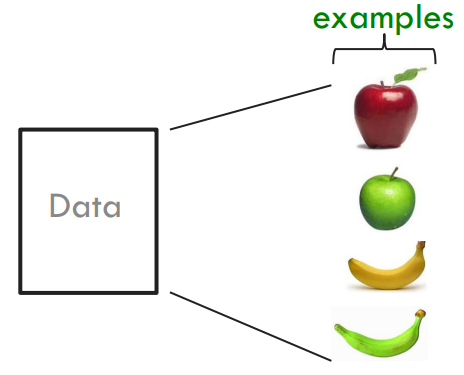
\includegraphics[width=0.35\textwidth]{006}
\end{wrapfigure}
Data are measured, collected, reported, and analyzed, and used to create data visualizations such as graphs, tables or images. Data as a general concept refers to the fact that some existing information or knowledge is represented or coded in some form suitable for better usage or processing.

We want to have a single way to treat our information and the same approach to represent the data. For each example in my training set, we have to translate these examples in terms of feature. Feature is usually a set of numbers, one example will be represented by a vector of cardinality \(N\).

\emph{Raw data} is a collection of numbers or characters before it has been \emph{cleaned} and corrected by researchers. Data processing commonly occurs by stages, and the processed data from one stage may be considered the raw data of the next stage.

Data is the most important part of all Data Analytics, Machine Learning, Artificial Intelligence. Without data, we can't train any model and all modern research and automation will go in vain.

\textbf{Information} is data that has been interpreted and manipulated and has now some meaningful inference for the user.

\textbf{Knowledge} is the combination of inferred information, experiences, learning, and insights. Results in awareness or concept building for an individual organization. Data can be split into:
\begin{itemize}
    \item \textbf{Training data}: the part of data we use to train our model. This is the data that the model actually sees (both input and output) and learns from.
    \item \textbf{Validation data}: the part of data that is used to do a frequent evaulation of the mode, fit on the training dataset along with improving involved hyperparameters (initially set parameters before the model begins learning). This data plays its part when the model is actually training.
    \item \textbf{Testing data}: once our model is completely trained, testing data provides an unbiased evaluation. When we feed in the inputs of testing data, our model will predict some values. After prediction, we evaluate our model by comparing it with the actual output present in the testing data. This is how we evaluate and see how much our model has learned from the experiences feed in as training data, set at the time of training. 
\end{itemize}

\subsection{Data Split}
Data is the information about the problem to solve in the form of a distribution, for classification and regression: \(p_{\text{data}} \in \Delta (X \times Y)\), for density estimation, clustering and dimensionality reduction: \(p_{\text{data}} \in \Delta (X)\). The data distribution \(p_{\text{data}}\) is typically unknown, but we can sample from it.

In machine learning, a common task is the study and construction of algorithms that can learn from and make predictions on data. Such algorithms function by making data-driven predictions or decisions, through building a mathematical model from input data. These input data used to build the model are usually divided in multiple data sets.

\subsubsection{Training set}
The model is initially fit on a \textbf{training data set}, which is a set of example used to fit the parameters of the model. The model is trained on the training set using a supervised learning method. In practice, the training set often consists of pairs of an input vector and the corresponding output vector, where the answer key is commonly denoted as the \emph{target}. The current model is run with the training set and produces a result, which is then compared with the target, for each input vector in the training set. Based on the result of the comparison and the specific learning algorithm being used, the parameters of the model are adjusted. The model fitting can include both variable selection and parameter estimation.

A training set is a set of examples used during the learning process and is used to fit the parameters of, for example, a classifier.

For classification tasks, a supervised learning algorithm looks at the training set to determina, or learn, the optimal combinations of variables that will generate a good predictive model. The goal is to produce a trained (fitted) model that generalizes well to new, unknown data. The fitted model is evaluated using new examples from the held-out datasets to estimate the model's accuracy in classifying new data. To reduce the risk of issues such as over-fitting, the examples in the validation and test datasets should not be used to train the model.

\begin{example}[Training set example]
\begin{wrapfigure}{l}{0.25\textwidth}
\begin{center}
    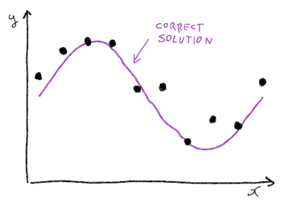
\includegraphics[width=0.25\textwidth]{017}
    \label{fig:017}
\end{center}
\end{wrapfigure}
Given the data \(D_n=\{(x_1,y_1),...,(x_n,y_n)\}\) generated from \(\sin(2 \pi x) + \)noise.\\
\\
The training set is made of pair, and is represented by \(n=10\) black dots. In the left figure we can see a graphical representtion of the training set. This data could serve for a task of regression.

\end{example}

\subsubsection{Validation test}
A \textbf{validation set} is a date set of examples used to tune the hyperparameters\footnote{\textbf{Hyperparameter:}  parameter whose value is used to control the learning proces. An example for artificial neural networks includes the number of hidden units in each layer.} of a classifier. It should follow the same probability distribution as the training set.

In order to avoid overfitting, when any classification parameter needs to be adjusted, it is necessary to have a validation set in addition to the training and test set. For example, if the most suitable classifier for the problem is sought, the training data set is used to train the different candidate classifiers, the validation data set is used to compare their performances and decide which one to take and, finally, the test set is used to obtain the performance characteristics such as accuracy, sensitivity, specificity, and so on. The validation set functions as a hybrid: it is training data used for testing, but neither as part of the low-level training nor as part of the final testing.

\subsubsection{Test set}
The \textbf{test data set} is a data set used to provide an unbiased evaluation of a final model fit on the training set. If the data in the test set has never been used in training, the test set is also called \textbf{holdout set}.

A test set is a data set that is independent of the training set, but that follows the same probability distribution. If a model fit to the training set also fits the test set well, minimal overfitting has taken place. A better fitting of the training data set as opposed to the test set usually points to over-fitting.

A test set is therefore a set of examples used only to assess the performance of a fully specified classifier. To do this, the final model is used to predict classifications of examples in the test set. Those predictions are compared to the examples' true classifications to assess the model's accuracy.

\begin{figure}[h]
\begin{center}
    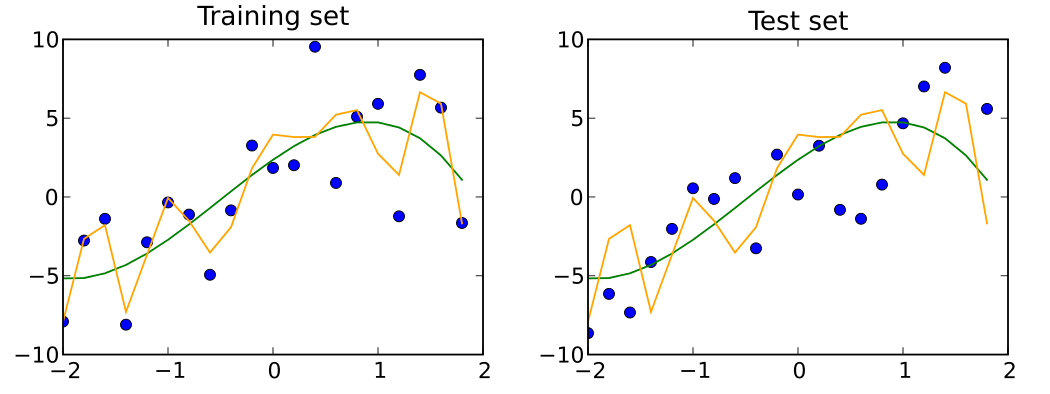
\includegraphics[width=.75\textwidth]{013}
    \caption{}
\end{center}
\caption{A training set and a test set from the same statistical population are shown as points. Two predictive models are fit to the training data. Both fitted models are plotted with both the training and test sets.}
\end{figure}

\subsection{Data generating distribution}
Our assumption is that learning problems are characterized by some unknown probablity distribution \(D\) over an input/output pairs \((x,y) \in X \times Y\). 

The training and test data are generated by a probability distribution overdatasets called the \textbf{data-generating process}. We typically make a set of assumptions known collectively as the i.i.d. assumptions. These assumptions are that the examples in each dataset are independent from each other, and thatthe training set and test set are identically distributed, drawn from the same probability distribution as each other. 

This assumption enables us to describe the data-generating process with a probability distribution over a single example. The same distribution is then used to generate every train example and every testexample. We call that shared underlying distribution the \textbf{data-generating distribution}, denoted \(p_data\). This probabilistic framework and the i.i.d. assumptions enables us to mathematically study the relationship between training error and test error.
\begin{figure}[h]
\begin{center}
    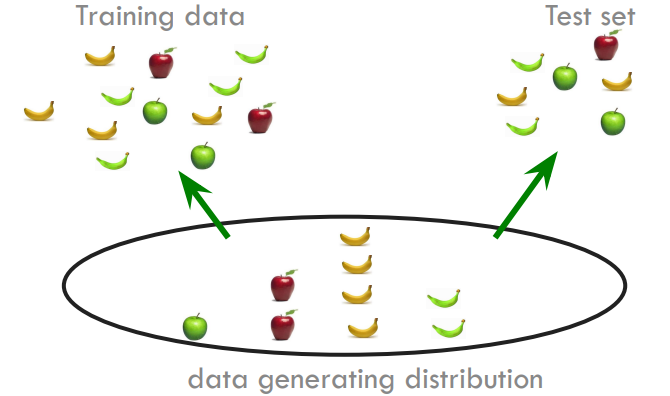
\includegraphics[width=.5\textwidth]{014}
    \caption{}
\end{center}
\caption{Example of a data generating distribution.}
\end{figure}


\section{Feature}
In machine learning and pattern recognition, a \textbf{feature} is an individual measurable property or characteristic of a phenomenon. Choosing informative, discriminating and independent features is a crucial element of effective algorithms in pattern recognition, classification and regression. Feature are usually numeric, but structural feature such as strings and graphs are used in syntactic pattern recognition. The concept of feature is related to that of explanatory variable used in statistical techniques such as linear regression.

\begin{wrapfigure}{l}{0.25\textwidth}
    \begin{center}
      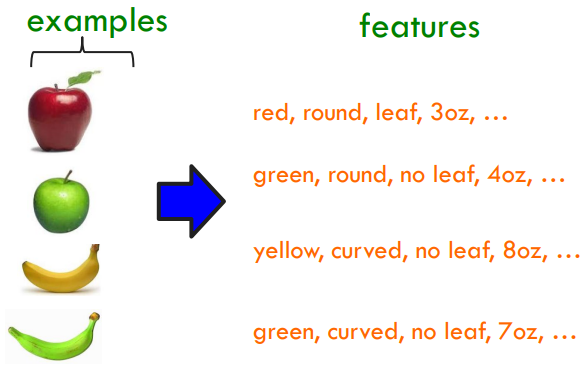
\includegraphics[width=0.25\textwidth]{007}
    \end{center}
\end{wrapfigure}

One of the most important aspect of machine learning model is identifying the features which will help create a great model, the model that performs well on unseen data. The initial set of raw features can be redundant and too large to be managed. Therefore, a preliminary step in many applications of machine learning and pattern recognition consists of selecting a subset of features, or constructing a new and reduced set of features to facilitate learning, and to improve generalization and interpretability. Extracting or selecting features is a combination of art and science; developing systems to do so is known as feature engineering. It requires the experimentation of multiple possibilities and the combination of automated techniques with the intuition and knowledge of the domain expert. Automating this process is feature learning, where a machine not only uses features for learning, but learns the features itself.

A \textbf{feature vector} is an \(n\)-dimensional vector of numerical features that represent some object. Many algorithms in machine learning require a numerical representation of objects, since such representations facilitate processing and statistical analysis. Feature vectors are often combined with weights using a dot product in order to construct a linear predictor function that is used to determine a score for making a prediction.

The vector spaces associated with these vector is often called \textbf{feature space}. In order to reduce the dimensionality of the feature space, a number of dimensionality reduction techniques can be employed.

Higher-level features can be obtained from already available features and added to the feature vector. This process is referred to as feature construction. Feature construction is the application of a set of constructive operators to a set of existing features resulting in construction of new features. Feature construction has long been considered a powerful tool for increasing both accuracy and understanding of structure, particularly in high-dimensional problems.

\subsection{Characteristics of good features}
A great feature must satisfy the following criteria, that are the characteristics of good features:
\begin{itemize}[topsep={0pt}, partopsep={0pt}]
    \item Features must be found in most of the data samples: Great features represent unique characteritistics which can be applied across different types of data samples and are not limited to just one data sample. For example, can the “red” color of apple act as a feature? Not really. Because apple can be found in different colors. It might have happened that the sample of apples that was taken for evaluation contained apple of just “red” color. If not found, we may end up creating models having high bias. 
    \item Features must be unique and may not be found prevalent with other (different) forms: Great features are the ones which is unique to apple and should not be applicable for other fruits. The toughness characteristic of apple such as “hard to teeth” may not be good feature. This is because a guava can also be explained using this feature. 
    \item Features in reality: There can be features which can be accidental in nature and is not a feature at all when considering the population. For example, in a particular sample of data, a particular kind of feature can be found to be prevalent. However, when multiple data samples are taken, the feature goes missing. 
\end{itemize}

\begin{figure}[t!]
    \begin{center}
        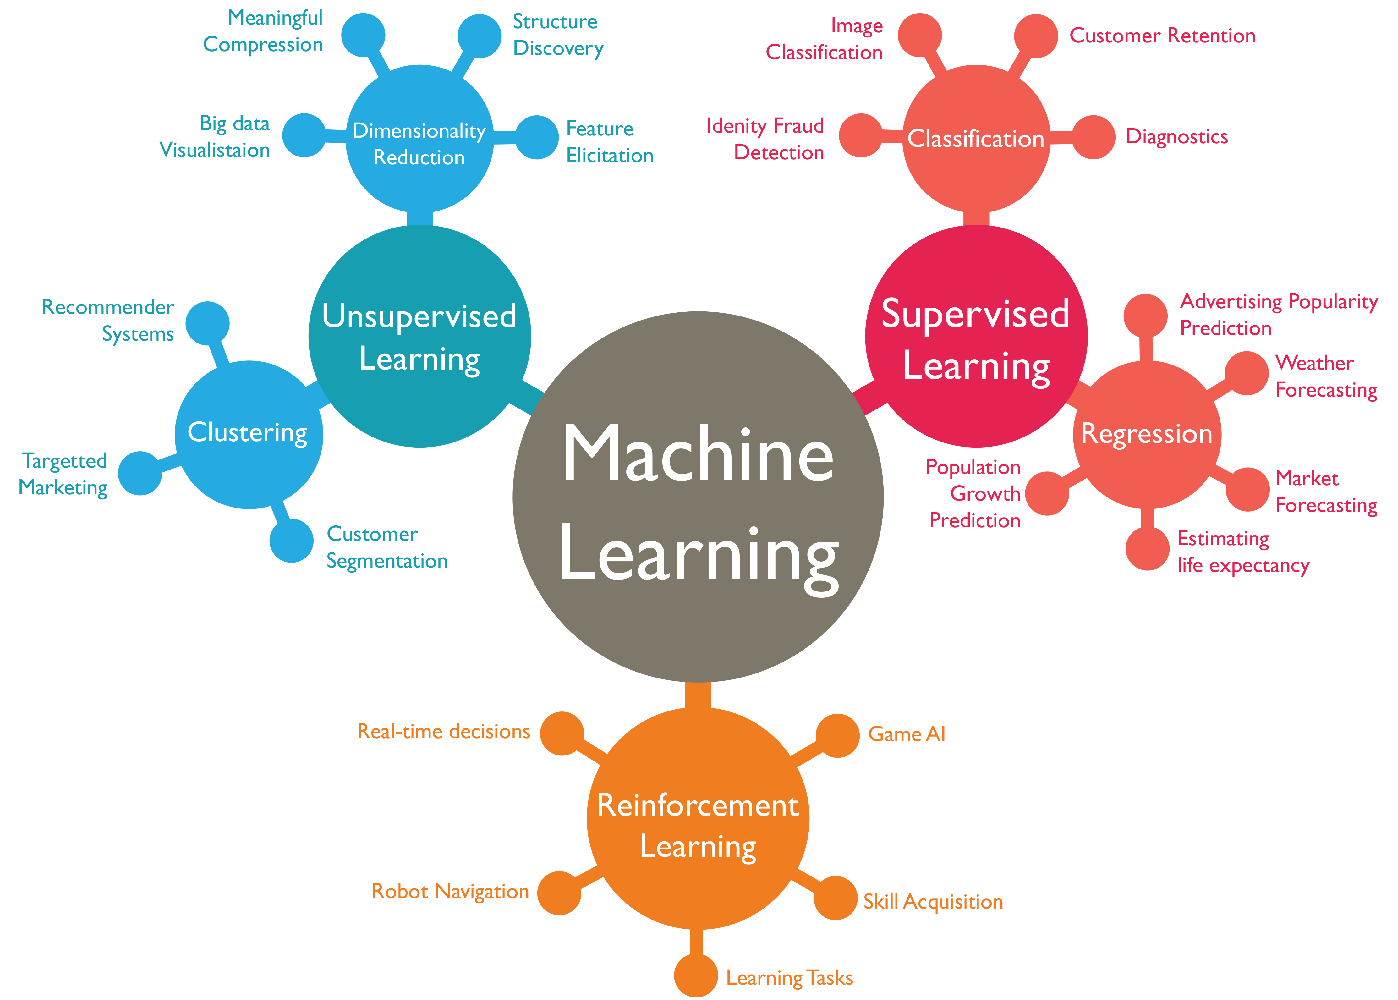
\includegraphics[width=\textwidth]{037}
    \end{center}
    \caption{Types of learning map}
    \label{fig:037}
\end{figure}

\section{Types of learning}
Machine learning approeaches are traditionally divided into three broad categories, depending on the nature of the \emph{signal} or \emph{feedback} available to the learning system. Machine Learning has found its applications in almost every business sector. There are several algorithms used in machine learning that help you build complex models. Each of these algorithms in machine learning can be classified into a certain category.

There are primarily three types of machine learning:
\begin{itemize}[topsep={0pt}, partopsep={0pt}]
    \item Supervised Learning;
    \item Unsupervisde Learning;
    \item Reinforcement Learning.
\end{itemize}

\subsection{Supervised learning}
\begin{wrapfigure}{l}{0.25\textwidth}
      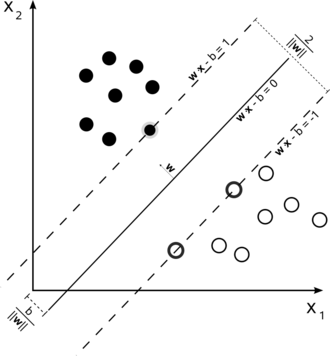
\includegraphics[width=0.25\textwidth]{008}
\end{wrapfigure}
Supervised learning algorithms build a mathematical model of a set of data that contains both the inputs and the desired outputs. The training data consists of a set of training examples. Each training example has one or more inputs and the desired output, also known as a supervisory signal. 

Through iterative optimization of an objective function, supervised learning algorithms learn a function that can be used to predict the ouput associated with new inputs. An optimal function will allow the algorithm to correctly determine the output for inputs that were not a part of the training data. An algorithm that improves the accuracy of its outputs or predictions over time is said to have learned to perform that task.

Supervised learning uses a training set to teach models to yield the desired output. This training dataset includes inputs and correct outputs, which allow the model to learn over time. The algorithm measures its accuracy through the loss function\footnote{We will talk more about loss functions in the next chapters.}, adjusting until the error has been sufficiently minimized.

We can resume the supervised learning in the following definition: Supervised learning is the machine learning task of learning a function that maps an input to an output based on example input-output pairs. It infers a function from labeled training data consisting of a set of training examples. In supervised learning, each example is a pair consisting of an input object (typically a vector) and a desired output value.

\subsubsection{Classification}
Classification is the problem of identifying which of a set of categories an observation belongs to. An algorithm that implements classification, especially in a concrete implementation, is known as a \emph{classifier}. The term also refers to the mathematical function, implemented by a classification algorithm, that maps input data to category.

Classification is a process of categorizing a given set of data into classes, It can be performed on both structured or unstructured data. The process starts with predicting the class of given data points. The classes are often referred to as target, label or categories.

The classification predictive modeling is the task of approximating the mapping function from input variables to discrete output variables. The main goal is to identify which class/category the new data will fall into.

We can divide the classification problem into two subproblems, that are binary classification and multiclass classification:
\begin{itemize}
\item \textbf{Binary classification: } It is a type of classification with two outcomes, for eg – either true or false. Given a training set \(T = \{(x_1,y_1), ..., (x_m, y_m)\}\). Learn a function \(f\) to predict \(y\) given \(x\). \(y\) is categorical, \(d=1\).
\[f: \mathbb{R}^d \to \{1,2,...,k\}\]
\item \textbf{Multiclass classification: } The classification with more than two classes, in multi-class classification each sample is assigned to one and only one label or target.. Given a training set \(T = \{(x_1,y_1), ..., (x_m, y_m)\}\). Learn a function \(f\) to predict \(y\) given \(x\). \(x\) is multidimensional (multiple features).
\[f: \mathbb{R}^d \to \{1,2,...,k\}\]
\end{itemize}

\begin{figure}[h!]
    \centering
    \begin{subfigure}{.4\textwidth}
        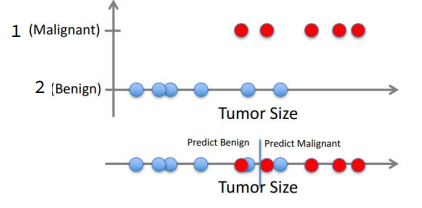
\includegraphics[width=1\textwidth]{009}
        \caption{Binary}
    \end{subfigure}
    \begin{subfigure}{.4\textwidth}
        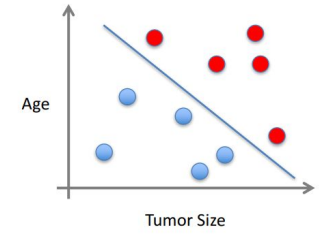
\includegraphics[width=1\textwidth]{010}
        \caption{Multiclass}
    \end{subfigure}
    \caption{Classification example}
\end{figure}

\begin{figure}[b]
    \centering
    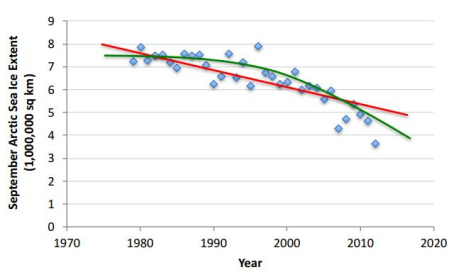
\includegraphics[width=.6\textwidth]{011}
    \caption{Regression}
\end{figure}

\subsubsection{Regression}
Regression analysis is a set of statistical processes for estimating the relationships between a dependent variable and one or more independent variables. The most common form of regression analysis is linear regression, in which one finds the line that most closely fits the data according to a specific mathematical criterion.

The following article provides an outline for Regression in Machine Learning. Regression means to predict the value using the input data. Regression models are used to predict a continuous value. It is mostly used to find the relationship between the variables and forecasting. Regression models differ based on the kind of relationship between dependent and independent variables.

Given a training set \(T = \{(x_1,y_1), ..., (x_m, y_m)\}\). Learn a function \(f\) to predict \(y\) given \(x\). \(y\) is real-valued \(d=1\).
\begin{equation}
    f: \mathbb{R}^d \to \mathbb{R}
\end{equation} 

Linear regression is employed in varied ways in which a number of them are listed as:
\begin{itemize}[topsep={0pt}, partopsep={0pt}]
\item Sales prognostication
\item Risk analysis
\item Housing applications
\item Finance applications
\end{itemize}

\subsubsection{Ranking}
Ranking is the data transformation in which numerical or ordinal values are replaced by their rank when the data are sorted.  Training data consists of lists of items with some partial order specified between items in each list. This order is typically induced by giving a numerical or ordinal score or a binary judgment (e.g. "relevant" or "not relevant") for each item. The goal of constructing the ranking model is to rank new, unseen lists in a similar way to rankings in the training data.

For example, the ordinal data \emph{hot}, \emph{cold}, and \emph{warm} would be replaced by \(3\), \(1\), \(2\).

\begin{example}
    Training data consists of queries and documents matching them together with relevance degree of each match. It may be prepared manually by human assessors (or raters, as Google calls them), who check results for some queries and determine relevance of each result. It is not feasible to check the relevance of all documents, and so typically a technique called pooling is used — only the top few documents, retrieved by some existing ranking models are checked. This technique may introduce selection bias. Alternatively, training data may be derived automatically by analyzing clickthrough logs (i.e. search results which got clicks from users), query chains, or such search engines' features as Google's (since-replaced) SearchWiki. Clickthrough logs can be biased by the tendency of users to click on the top search results on the assumption that they are already well-ranked.
\end{example}

\subsection{Unsupervised learning}
Unsupervised learning algorithms take a set of data that contains only inputs, and find structure in the data, like grouping or clustering of data points. The algorithms, therefore, learn from test data that has not been labeled, classified or categorized. 

Unsupervised learning uses machine learning algorithms to analyze and cluster unlabeled datasets. These algorithms discover hidden patterns or data groupings without the need for human intervention. Its ability to discover similarities and differences in information make it the ideal solution for exploratory data analysis, cross-selling strategies, customer segmentation, and image recognition.

Instead of responding to feedback, unsupervised learning algorithms identify commonalities in the data and react based on the presence or absence of such commonalities in each new piece of data.

\begin{figure}
    \begin{center}
        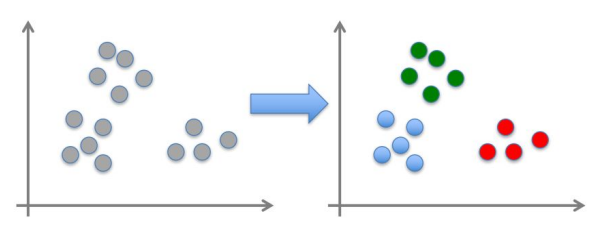
\includegraphics[width=.6\textwidth]{012}
    \end{center}
    \caption{Clustering}
    \end{figure}
    
\subsubsection{Clustering}
Cluster analysis is the assignment of a set of observations into subsets (called \emph{clusters}) so that observations within the same cluster are similar according to one or more predesignated criteria, while observations drawn from different clusters are dissimilar. 

Cluster analysis itself is not one specific algorithm, but the general task to be solved. It can be achieved by various algorithms that differ significantly in their understanding of what constitutes a cluster and how to efficiently find them. Popular notions of clusters include groups with small distances between cluster members, dense areas of the data space, intervals or particular statistical distributions. Clustering can therefore be formulated as a multi-objective optimization problem. The appropriate clustering algorithm and parameter settings (including parameters such as the distance function to use, a density threshold or the number of expected clusters) depend on the individual data set and intended use of the results. Cluster analysis as such is not an automatic task, but an iterative process of knowledge discovery or interactive multi-objective optimization that involves trial and failure. It is often necessary to modify data preprocessing and model parameters until the result achieves the desired properties.

Formally, given \(T = \{x_1, ..., x_m\}\) without labels, the output is the hidden structure behind the \(x\)'s, that is the cluster.

\subsubsection{Anomaly detection}
Anomaly detection is the identification of rare items, events or observations which raise suspicions by differing significantly from the majority of the data.
In data analysis, anomaly detection (also referred to as outlier detection) is generally understood to be the identification of rare items, events or observations which deviate significantly from the majority of the data. Such examples may arouse suspicions of being generated by a different mechanism, or appear inconsistent with the data.

Typically the anomalous items will translate to some kind of problem such as bank fraud, a structural defect, medical problems or errors in a text. Anomalies are also referred to as outliers, novelties, noise, deviations and exceptions.

Anomaly detection is applicable in a very large number and variety of domains, and is an important subarea of unsupervised machine learning. As such it has applications in cyber-security intrusion detection, fraud detection, fault detection, system health monitoring, event detection in sensor networks, detecting ecosystem disturbances, defect detection in images using machine vision, medical diagnosis and law enforcement.

\subsubsection{Dimensionality reduction}
Dimensionality reduction is a process of reducing the number of random variables under consideration by obtaining a set of principal variables. It is a process of reducing the dimension of the feature set, also called \emph{number of features}. Most of the dimensionality reduction techniques can be considered as either feature elimination or extraction.

Dimensionality reduction, or dimension reduction, is the transformation of data from a high-dimensional space into a low-dimensional space so that the low-dimensional representation retains some meaningful properties of the original data, ideally close to its intrinsic dimension. Working in high-dimensional spaces can be undesirable for many reasons; raw data are often sparse as a consequence of the curse of dimensionality, and analyzing the data is usually computationally intractable (hard to control or deal with). Dimensionality reduction is common in fields that deal with large numbers of observations and/or large numbers of variables, such as signal processing, speech recognition, neuroinformatics, and bioinformatics.

Dimensionality reduction can be used for noise reduction, data visualization, cluster analysis, or as an intermediate step to facilitate other analyses.

\subsection{Reinforcement learning}
Reinforcement learning is an area of machine learning concerned with how intelligent agents ought to take actions in an environment in order to maximize the notion of cumulative reward. 

Reinforcement learning is the training of machine learning models to make a sequence of decisions. The agent learns to achieve a goal in an uncertain, potentially complex environment. In reinforcement learning, an artificial intelligence faces a game-like situation. The computer employs trial and error to come up with a solution to the problem. To get the machine to do what the programmer wants, the artificial intelligence gets either rewards or penalties for the actions it performs. Its goal is to maximize the total reward.
Although the designer sets the reward policy-that is, the rules of the game-he gives the model no hints or suggestions for how to solve the game. It's up to the model to figure out how to perform the task to maximize the reward, starting from totally random trials and finishing with sophisticated tactics and superhuman skills. By leveraging the power of search and many trials, reinforcement learning is currently the most effective way to hint machine's creativity. In contrast to human beings, artificial intelligence can gather experience from thousands of parallel gameplays if a reinforcement learning algorithm is run on a sufficiently powerful computer infrastructure.
\begin{figure}[t!]
    \begin{center}
        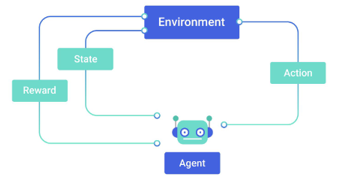
\includegraphics[width=.6\textwidth]{016}
    \end{center}
    \caption{Reinforcement learning flow chart}
    \label{fig:016}
\end{figure}

Training the models that control autonomous cars is an excellent example of a potential application of reinforcement learning. In an ideal situation, the computer should get no instructions on driving the car. The programmer would avoid hard-wiring anything connected with the task and allow the machine to learn from its own errors. In a perfect situation, the only hard-wired element would be the reward function.

\subsection{Other Learning Types}
- semi-supervised learning,
- active learning,
- online vs offline learning,
- generative vs discriminative,
- parametric vs non-parametric.

\newpage
\begin{exercise}[topsep=20pt,itemsep=10pt]
    \ex Describe the learning process and each of its step.
    \ex What is data? How can be split? How is it used in Machine Learning?
    \ex Provide the definitions of Information and Knowledge.
    \ex What is a feature? What is a feature vector? What do they represent? 
    \ex Provide the definitions of the three types of learning.
    \ex Provide the definitions of classification, regression, and ranking.
    \ex[!] What is multiclass classification?
    \ex Provide the definitions of clustering, anomaly detection, and dimensionality reduction.
    \ex[!] What is dimensionality reduction? What is it useful for? What are its benefits?
    \ex What is Reinforcement Learning? Provide a basic flow chart.
    \ex[!] What is the difference between supervised learning and reinforcement learning?
\end{exercise}